% Chapter 1

\chapter{Hardware Architecture for Inter-Prediction} % Write in your own chapter title
\label{Chapter4}
\lhead{Chapter 4. \emph{Hardware Architecture for Inter-Prediction}} % Write in your own chapter title to set the page header

There are many new technologies such as intra prediction, in-loop deblocking filter and context based arithmetic coding introduced in the latest H.264/AVC standard. Among all of these amazing technologies, \textbf{Variable Block Size Motion Estimation (VBSME)} is one of the most powerful techniques. In comparison with the previous Fixed Block Size Motion Estimation (FBSME), VBSME divides one MB into smaller blocks to fit different motion directions. In this way, the coding performance is proved.

\subsection{Full Search ME Algorithm}
The Full Search Algorithm works in the following way:
\begin{itemize}
	\item At first, both the search window and current block positions are fixed at the certain point i.e top left corner of frame. The current block starts the loading of the pixels from the top left corner. Absolute difference of each pixel of current block with the corresponding pixel of the search window is calculated.
	\begin{equation} \label{equ:1}
		Diff(m,n,k,l\ = |S(m+k, n+l) - C(k,l)|
	\end{equation}
	\item After that the Sum of all Absolute Differences (SAD) for that particular position of current block is calculated.
	\begin{equation} \label{equ:2}
		SAD(m,n) = \sum_{k=0}^{W-1}\sum_{l=0}^{H-1}Diff(m,n,k,l) 
	\end{equation}
	Then the current block is shifted by 1 row or column of pixels and again SAD is calculated. In this way, several SADs are calculated in a single search window.
	\item Each SAD when calculated is compared with the previous SAD value and the smaller SAD value is taken. In this way at end, minimum SAD value and the corresponding motion vectors values are depicted for one search window. 
	\begin{equation} \label{equ:3}
		SAD_{min} = min(SAD(m,n))
	\end{equation}
\end{itemize}

In the above equation (\ref{equ:1}), (\ref{equ:2}) and (\ref{equ:3}) The domain of m and n is $m \in [0, M-1] $ and $m \in [0, N-1]$ respectively.M and N are width and height of search window respectively. H and W are height and width of current block respectively. C(k,l) represents the pixel value of the current block and S(m+k, n+l) is the pixel value from the search window of the reference frame.\cite{li2003serial} \\

\subsection{256 PE VBS FS ME Hardware Architecture}
We designed a parallel \textbf{256 PE VBS FSME Hardware Architecture}. \cite{kalaycioglu2011low} This hardware is implemented in System Verilog. First of all, the pixels in the current MB are stored in a Block Ram \textbf{(c$\_$BRAM)}. The pixels of the search window are also stored in a block RAM \textbf{(s$\_$BRAM)}. The architecture is shown in the figure \ref{fig:256pevbsme}

\begin{figure}[htbp]
	\centering
	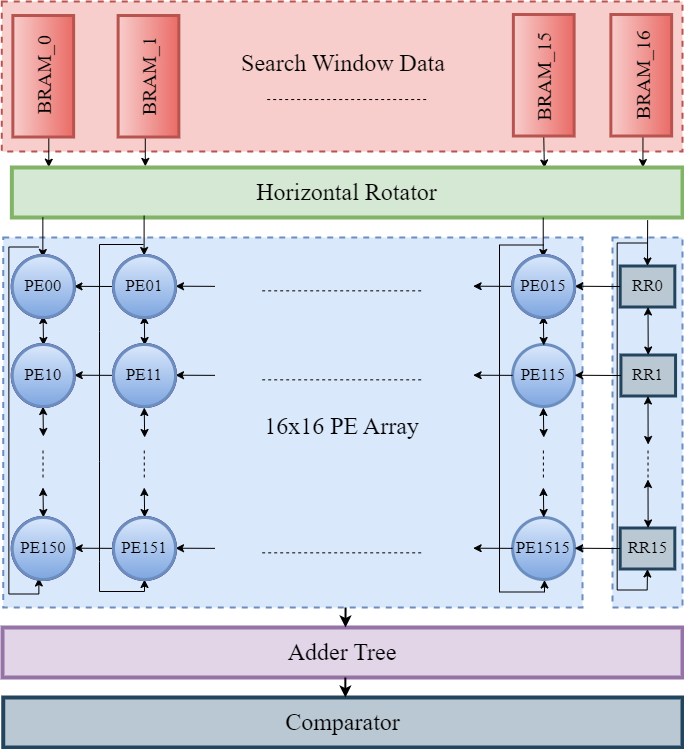
\includegraphics[width = 4in]{./Figures/256pevbsme.png}
	\rule{35em}{0.5pt}
	\caption{265 PE VBS ME Hardware Architecture}
	\label{fig:256pevbsme}
\end{figure}

In this design, a \textbf{2-D systolic PE array} is used. The use of this type of array introduced parallel computing and pipelinability in the structure. There are \textbf{16x16 = 256 PEs} ( 16 rows and 16 columns) interconnected with each other in a form of matrix. All of them are  made capable of shifting data down, up and left. It means that a 16x16 current block can move around the 48x48 search window in down, up and right direction. For a \textbf{16x16 MB}, a Motion Vector MV is found in one cycle in a search range of \textbf{[-16, 15]} pixels. Pixels are defined as 8 bit positive integers.

As soon as the control signals for loading current and search pixels are enabled, both current block and search window pixels starts loading into PEs. In 1 clock cycle, 16 pixels are loaded for both of them. (1st PE is filled in each of 16 columns). Thus, the whole PE matrix is filled in 16 cycles. As depicted in figure \ref{fig:pematrix}, \textbf{pixel$\_$cpr$\_$in} and \textbf{pixel$\_$spr$\_$in} are input array of 16 8-bit pixels from current block and search window of reference block respectively. The \textbf{pe$\_$}matrix module concatenates the output signals of each column of processing elements to form the final output signal \textbf{ad} which is an array of 8*(16**2) bits. 

\begin{figure}[htbp]
	\centering
	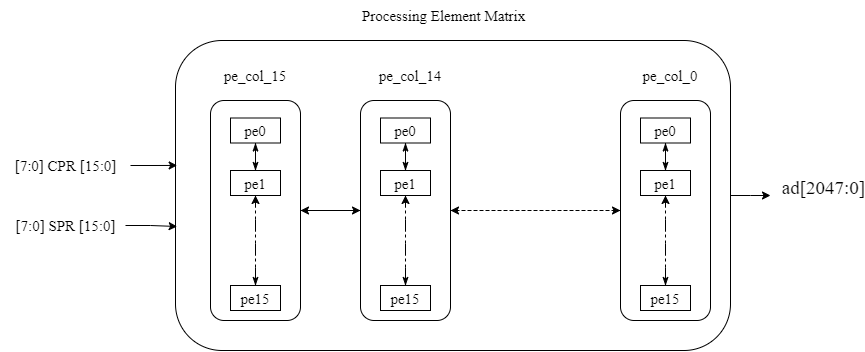
\includegraphics[width = 4.5in]{./Figures/pematrix.png}
	\rule{35em}{0.5pt}
	\caption{16 x 16 PE Matrix}
	\label{fig:pematrix}
\end{figure}

Each PE calculates the absolute difference between current MB pixel and the search window pixel. In this way 16x16 = 256 absolute differences are obtained in one location and they all are calculated simultaneously with the loading of data in PEs as the design is combinational. 

After absolute differences are all calculated, The SAD for that search location is determined by adding the absolute differences calculated by the above PEs as shown in figure. All these absolute differences are added up together using Adder Trees. The working of a simple adder tree is shown in figure \ref{fig:addertree}. It can seen clearly in the figure that there is 2 cycle latency for an adder tree. 

\begin{figure}[htbp]
	\centering
	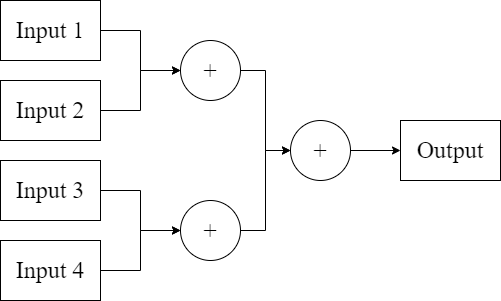
\includegraphics[width = 2in]{./Figures/addertree.png}
	\rule{35em}{0.5pt}
	\caption{Working of an Adder Tree}
	\label{fig:addertree}
\end{figure}

For SAD calculation of a 16x16 current block, we consider \textbf{PI-PPSAD} structure.  

